\documentclass[letterpaper,12pt]{article}
\usepackage{tabularx} % extra features for tabular environment
\usepackage{amsmath}  % improve math presentation
\usepackage{float}
\usepackage{pdfpages}
\usepackage{steinmetz}

\usepackage{graphicx} % takes care of graphic including machinery
\graphicspath{ {./figures/} }
\usepackage[margin=1in,letterpaper]{geometry} % decreases margins
\usepackage{cite} % takes care of citations
\usepackage[final]{hyperref} % adds hyper links inside the generated pdf file
\hypersetup{
	colorlinks=true,       % false: boxed links; true: colored links
	linkcolor=blue,        % color of internal links
	citecolor=blue,        % color of links to bibliography
	filecolor=magenta,     % color of file links
	urlcolor =blue         
}




\begin{document}

\title{Experiment 4 Preliminary Work \protect\\ Impedance Measurement and  Complex Power}
\author{Ahmet Akman 2442366 \protect\\}
\date{\today}
\maketitle
\tableofcontents
%\begin{abstract}
%abstract
%\end{abstract}

%\section{Introduction}
\section{Step 1}
In this step the circuits given in Figure 1 is taken as the reference.
\begin{figure}[H]
    \centering
    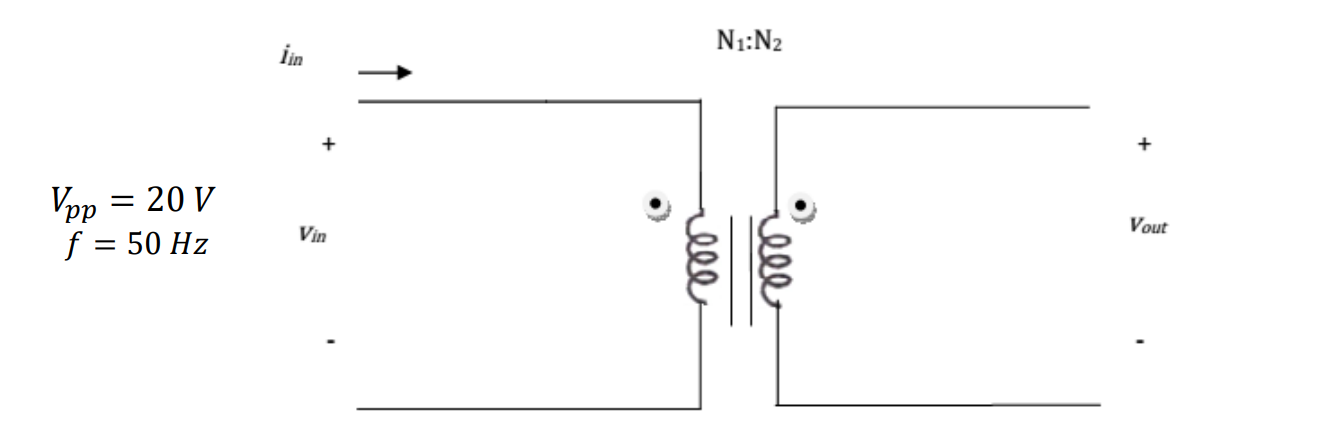
\includegraphics[width=1\textwidth]{1.png}
    \caption{Circuit schematic for the step 1}
\end{figure} 

\subsection{a)}
The circuit given in Figure 2 is constructed in LTSpice environment.
\begin{figure}[H]
    \centering
    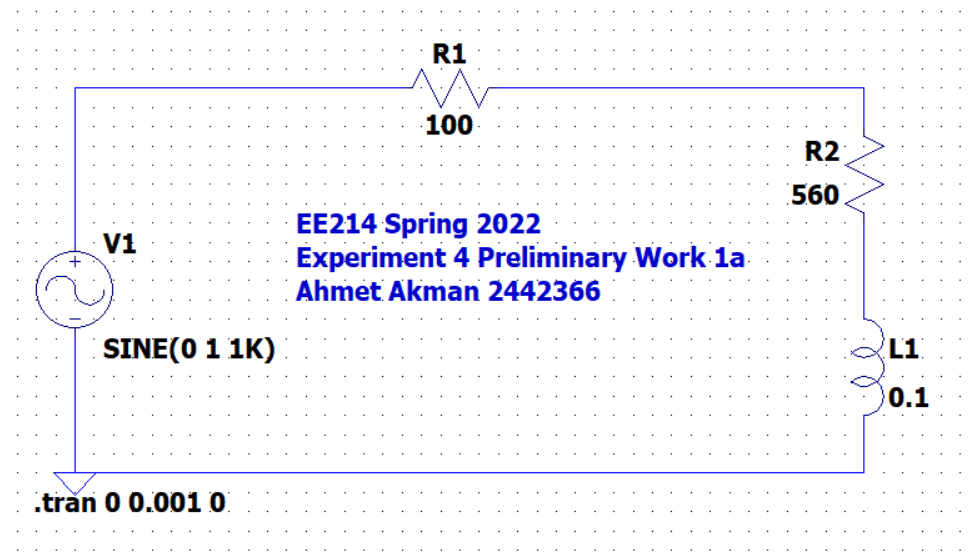
\includegraphics[width=1\textwidth]{1aSCH.png}
    \caption{Circuit schematic in LTSpice for the step 1 part a}
\end{figure} 
As a result the plot of voltage and current characteristics of input and load are given in Figure 3.
\begin{figure}[H]
    \centering
    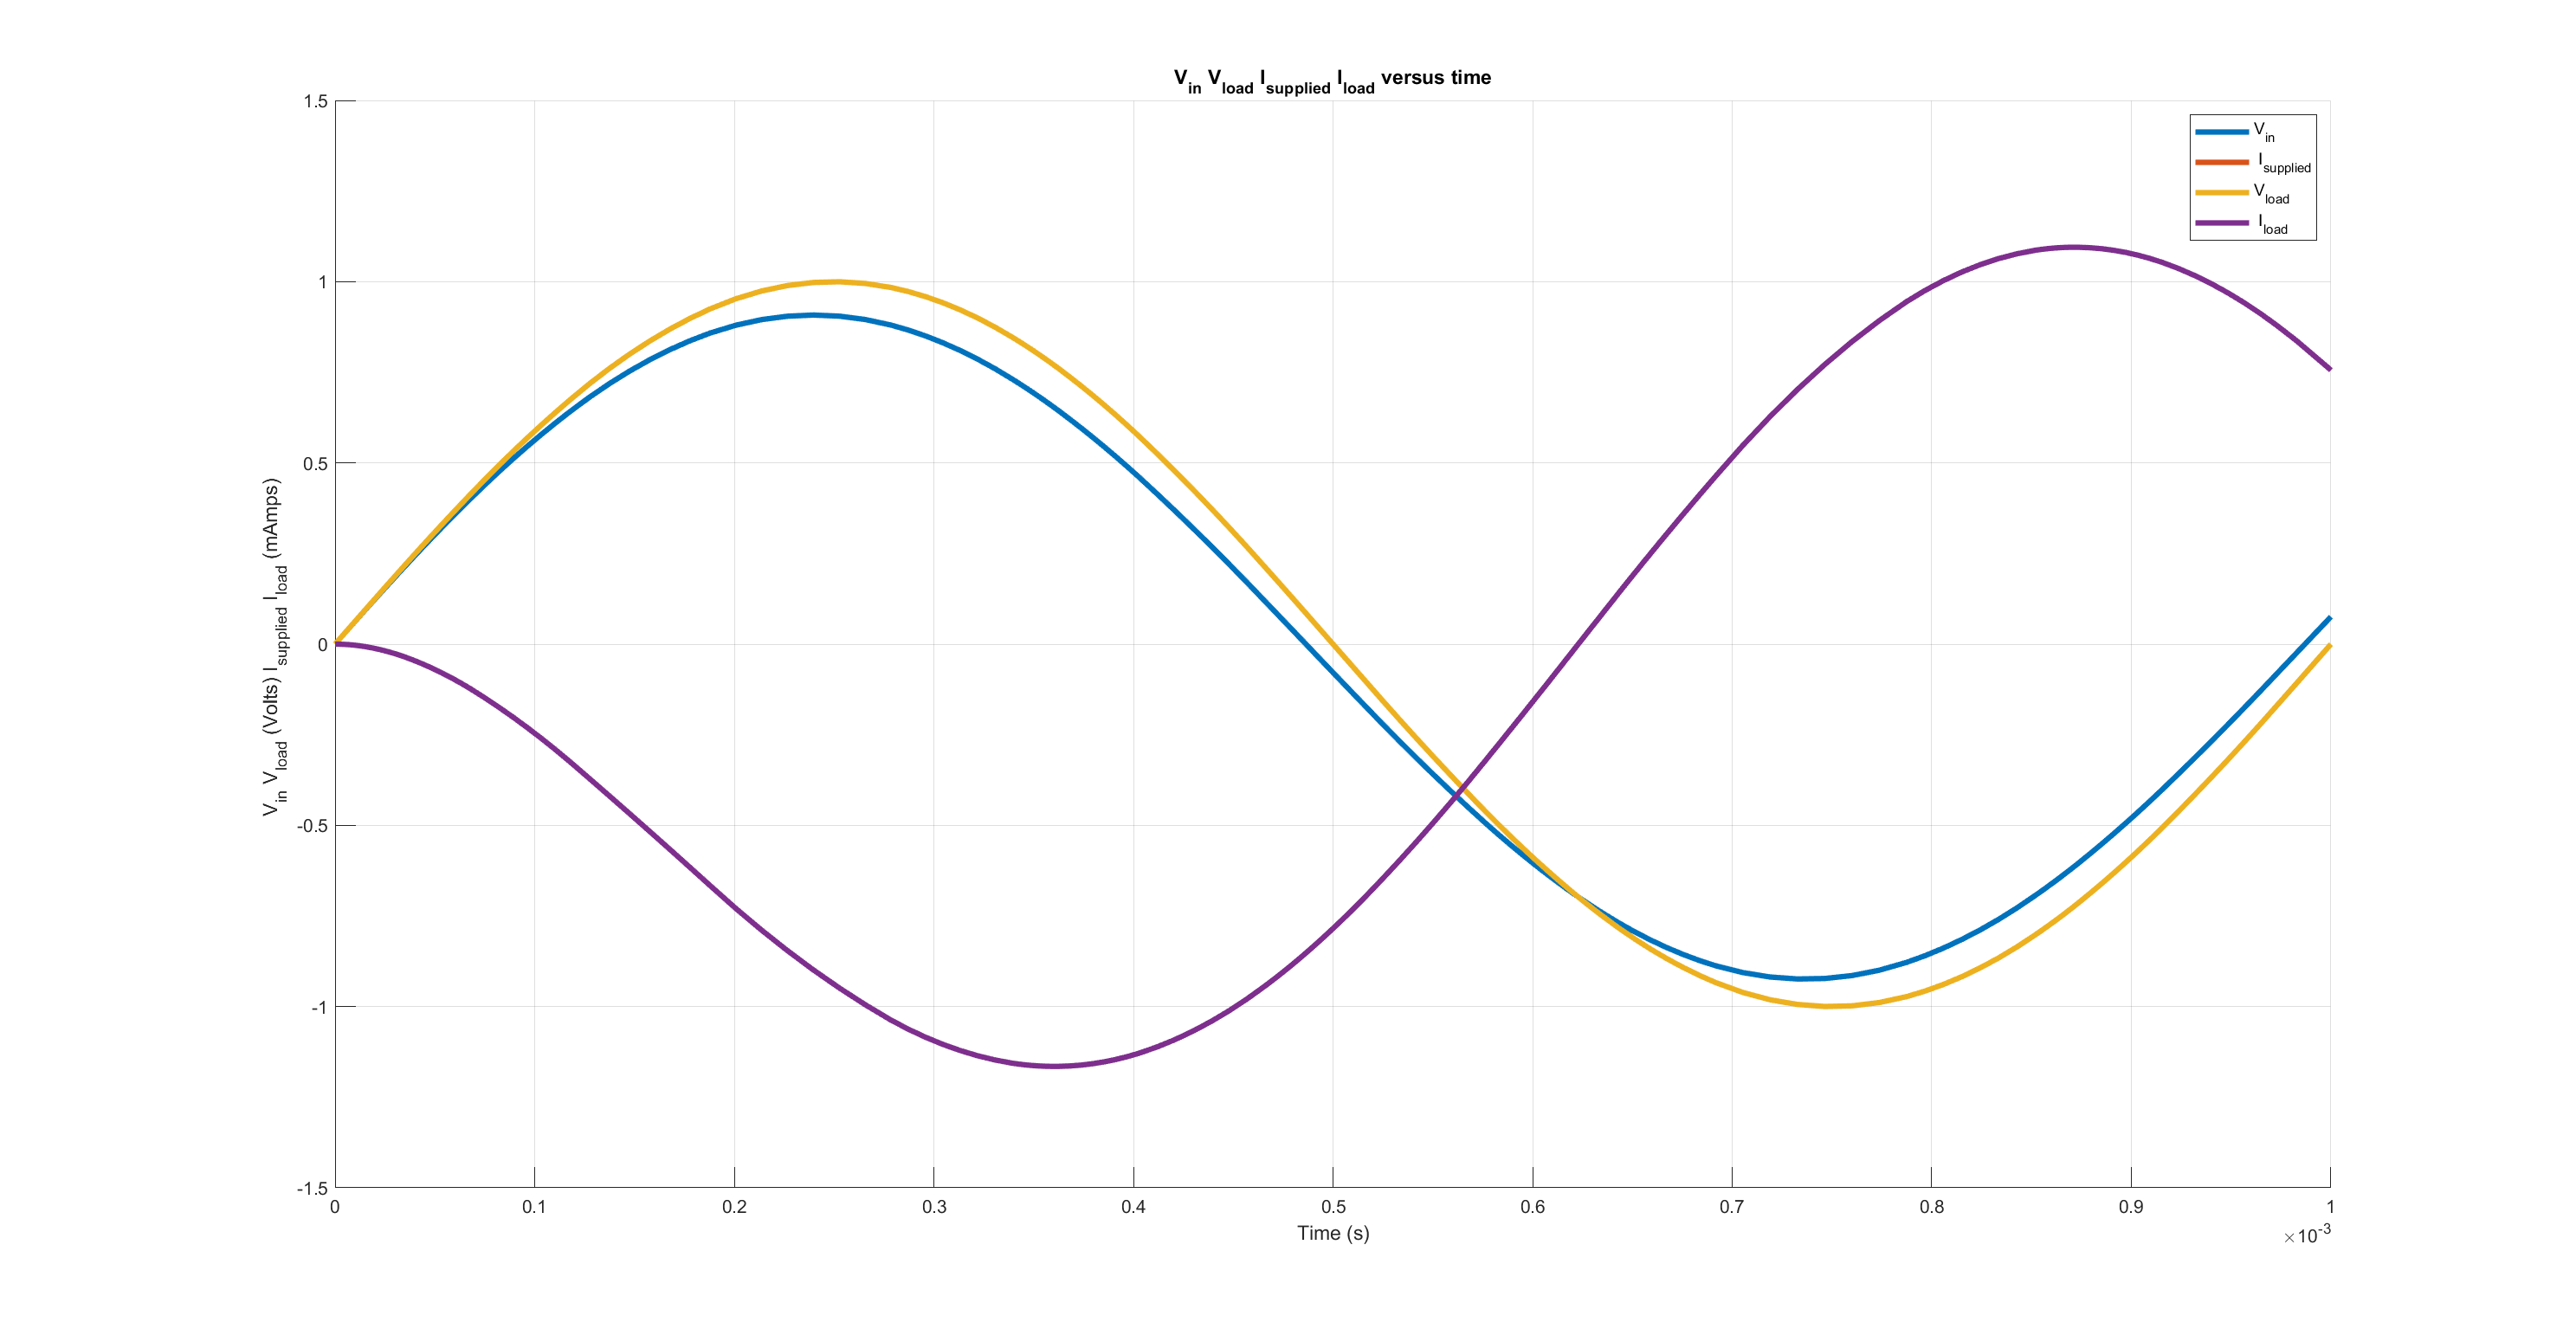
\includegraphics[width=1\textwidth]{1_1.png}
    \caption{I and V versus time for Input and Load}
\end{figure} 
To obtain power consumed at load, \(IR2\) and \(V_{load}\) are multiplied. The plot given in Figure 4 is obtained.
\begin{figure}[H]
    \centering
    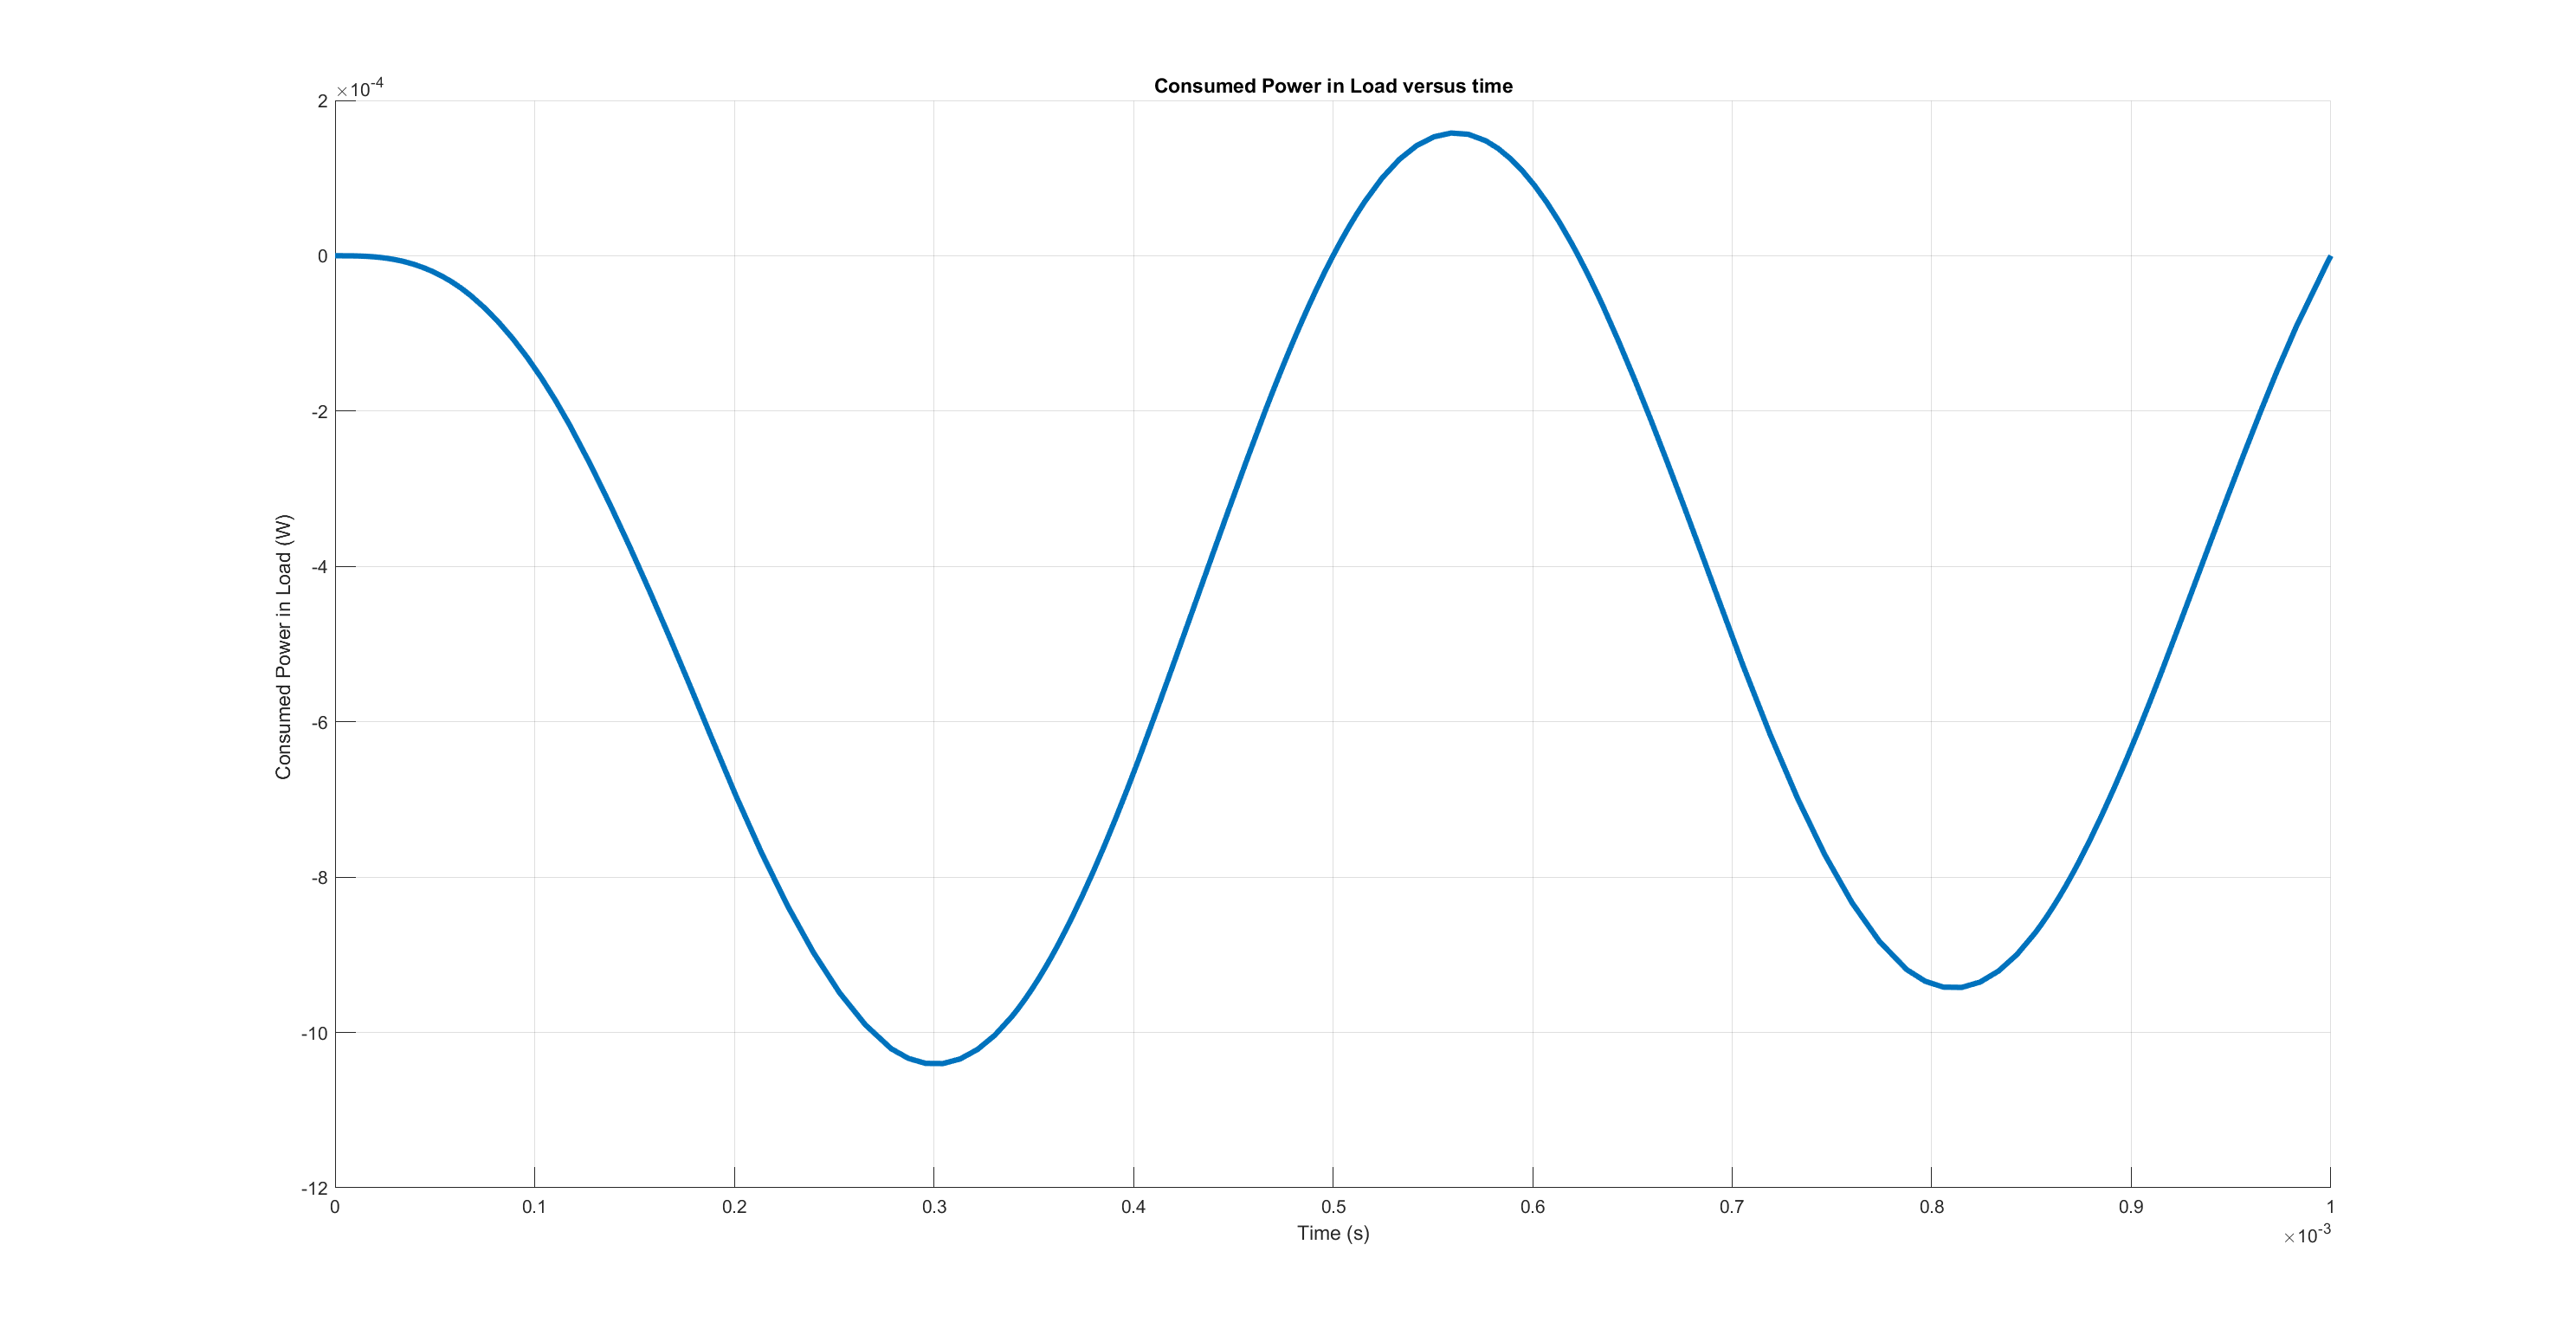
\includegraphics[width=1\textwidth]{1_2.png}
    \caption{Power consumed at load versus Time}
\end{figure} 
The average and the RMS values of the load power are calculated and given in Table 1.
\begin{table}[H]
    \begin{center}
        \caption{Resistance reading by color code convention.}
        \vspace{2mm}
        \begin{tabular}{||c | c ||} 
            \hline
            Average (W) & RMS (W) \\ [0.5ex] 
            \hline\hline
            \(-3.61x10^{-4}\) & \(5.37x10^{-4}\)  \\ 
            \hline
    \end{tabular}
\end{center}
\end{table}

\subsection{b)}
The circuit given in Figure 5 is constructed in LTSpice environment. In addition to previous step a capacitor with 100nF is connected.
\begin{figure}[H]
    \centering
    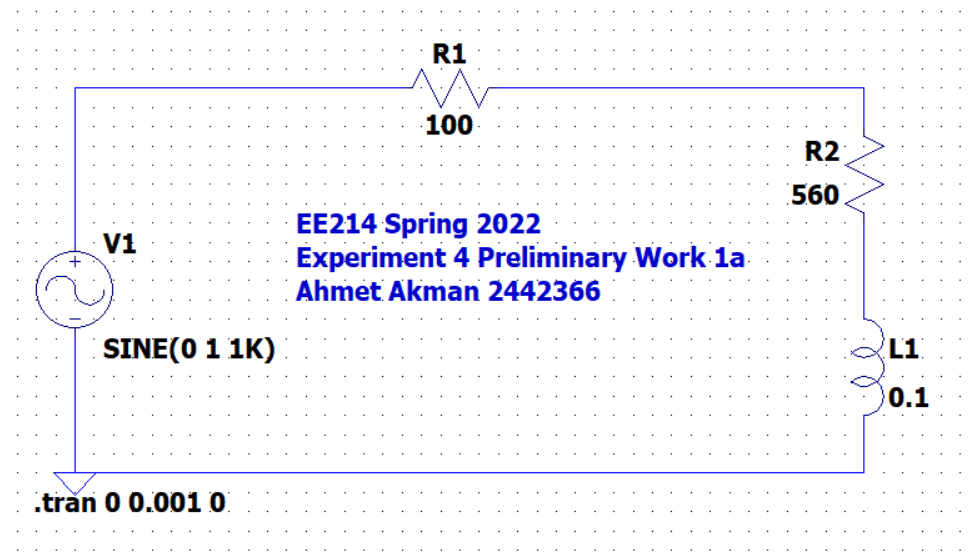
\includegraphics[width=1\textwidth]{1aSCH.png}
    \caption{Circuit schematic in LTSpice for the step 1 part b}
\end{figure} 
As a result the plot of voltage and current characteristics of input and load are given in Figure 6.
\begin{figure}[H]
    \centering
    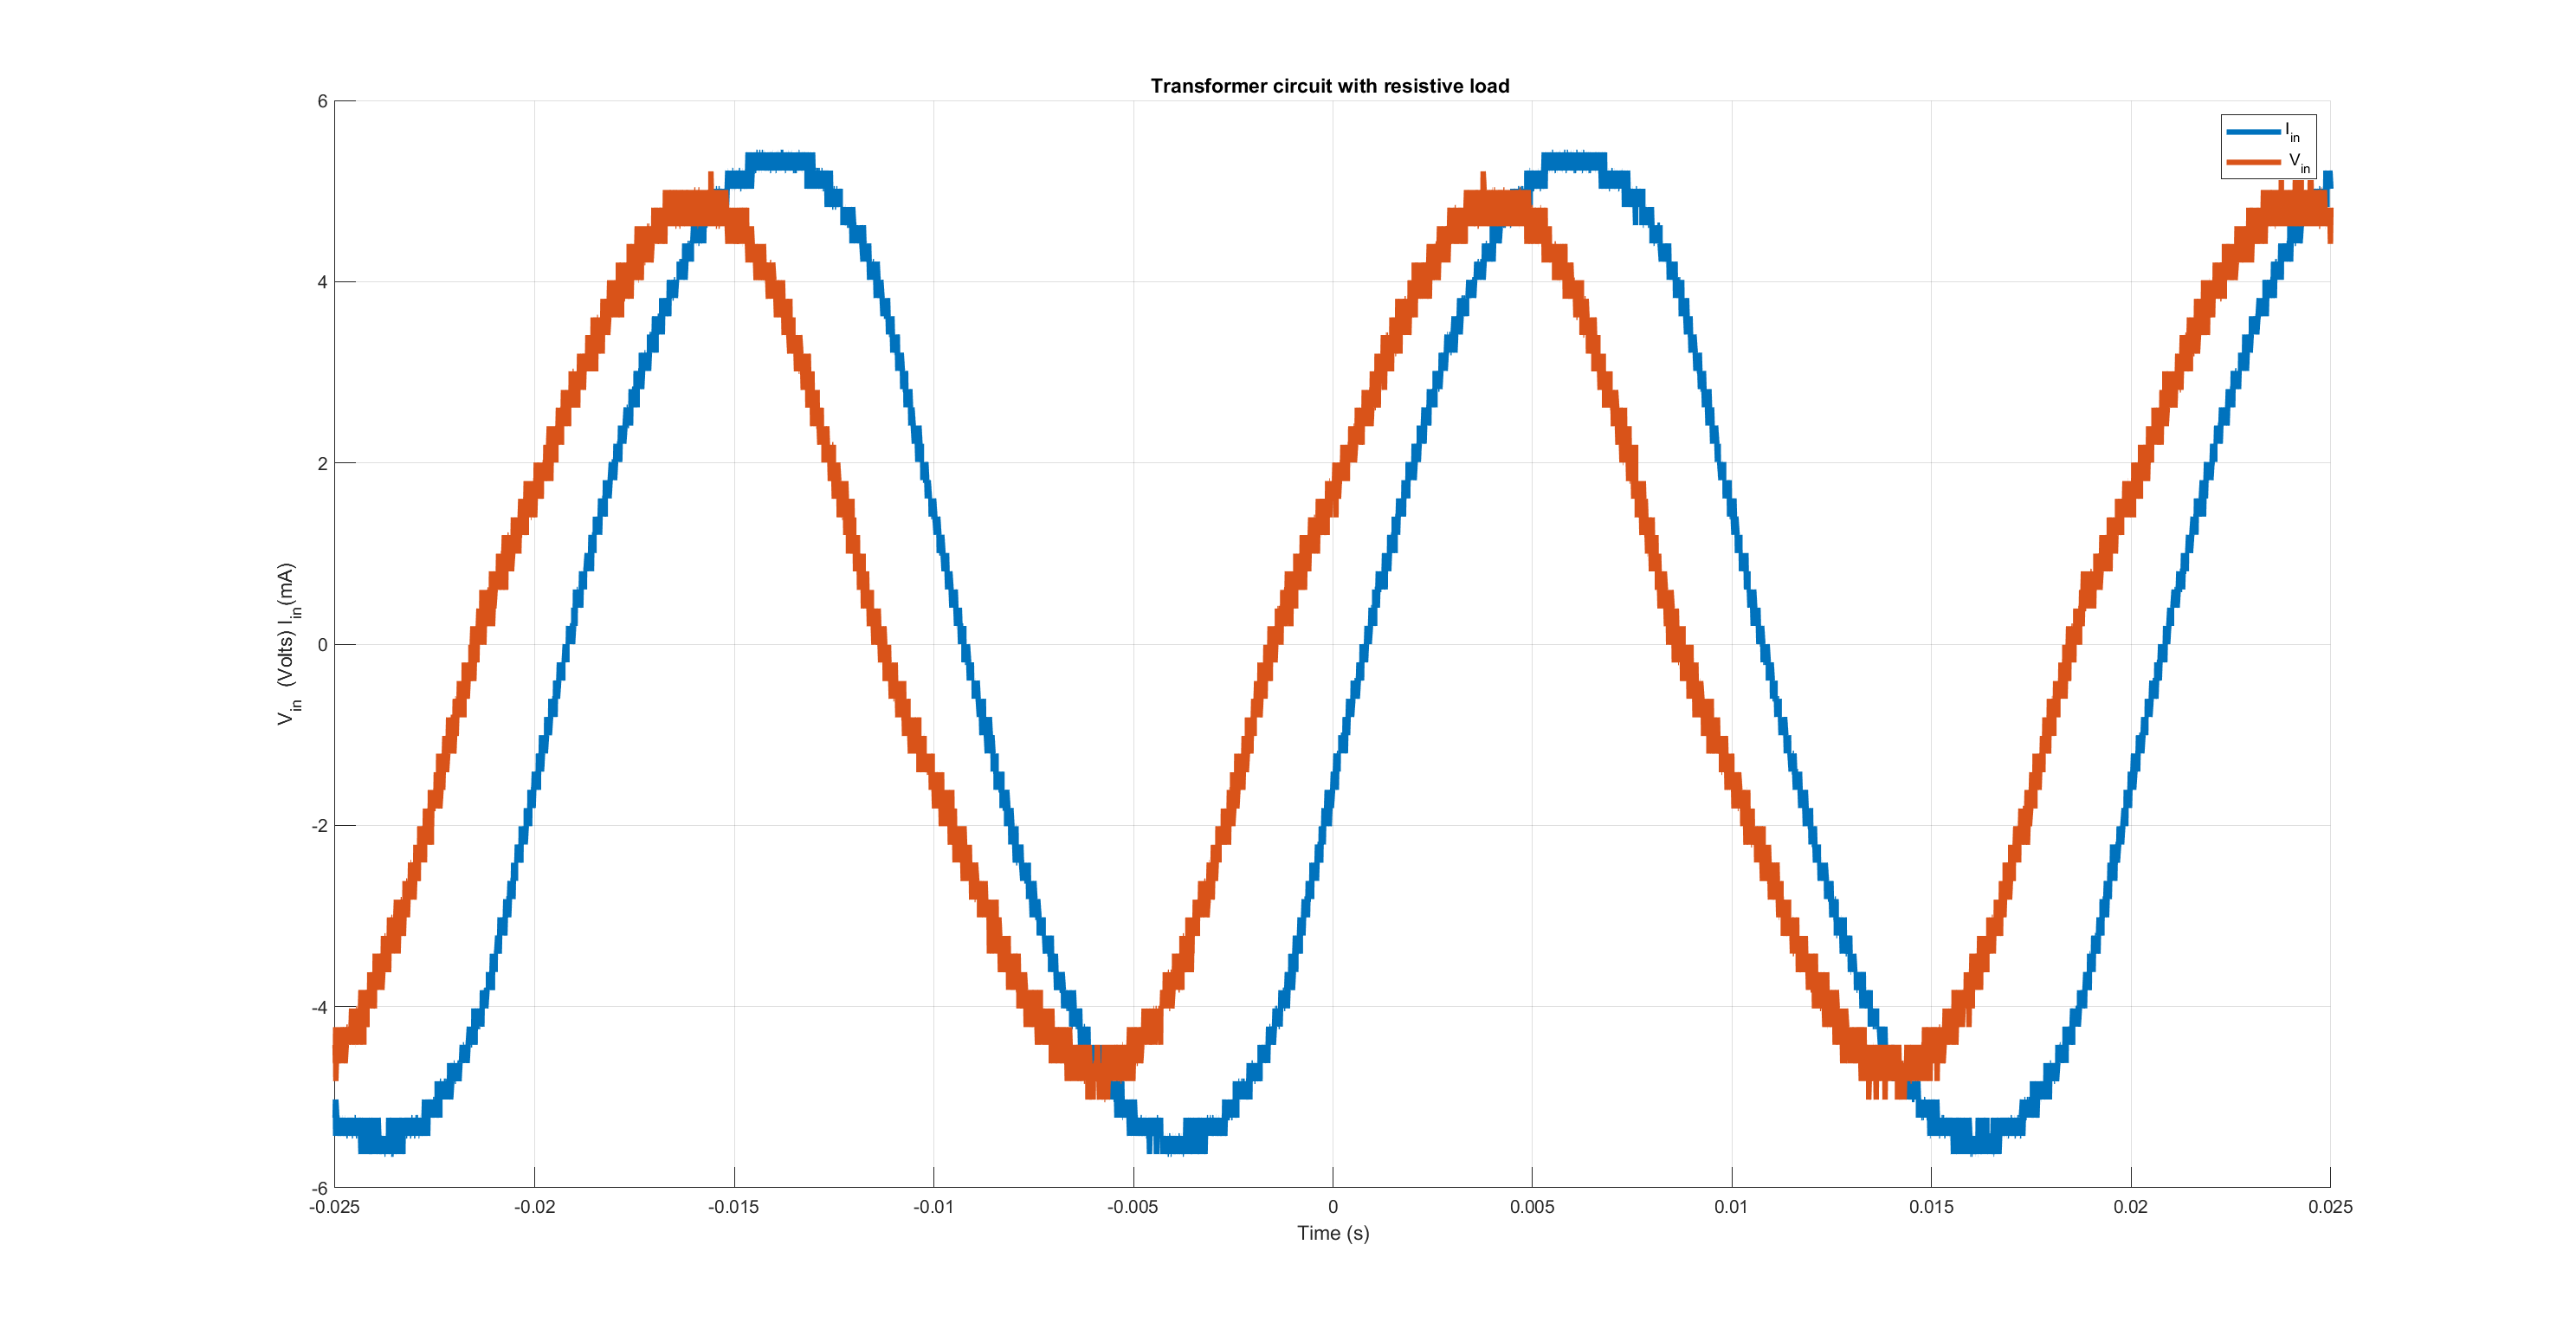
\includegraphics[width=1\textwidth]{2_1.png}
    \caption{I and V versus time for Input and Load}
\end{figure} 
To obtain power consumed at load, \(IR2\) and \(V_{load}\) are multiplied. The plot given in Figure 7 is obtained.
\begin{figure}[H]
    \centering
    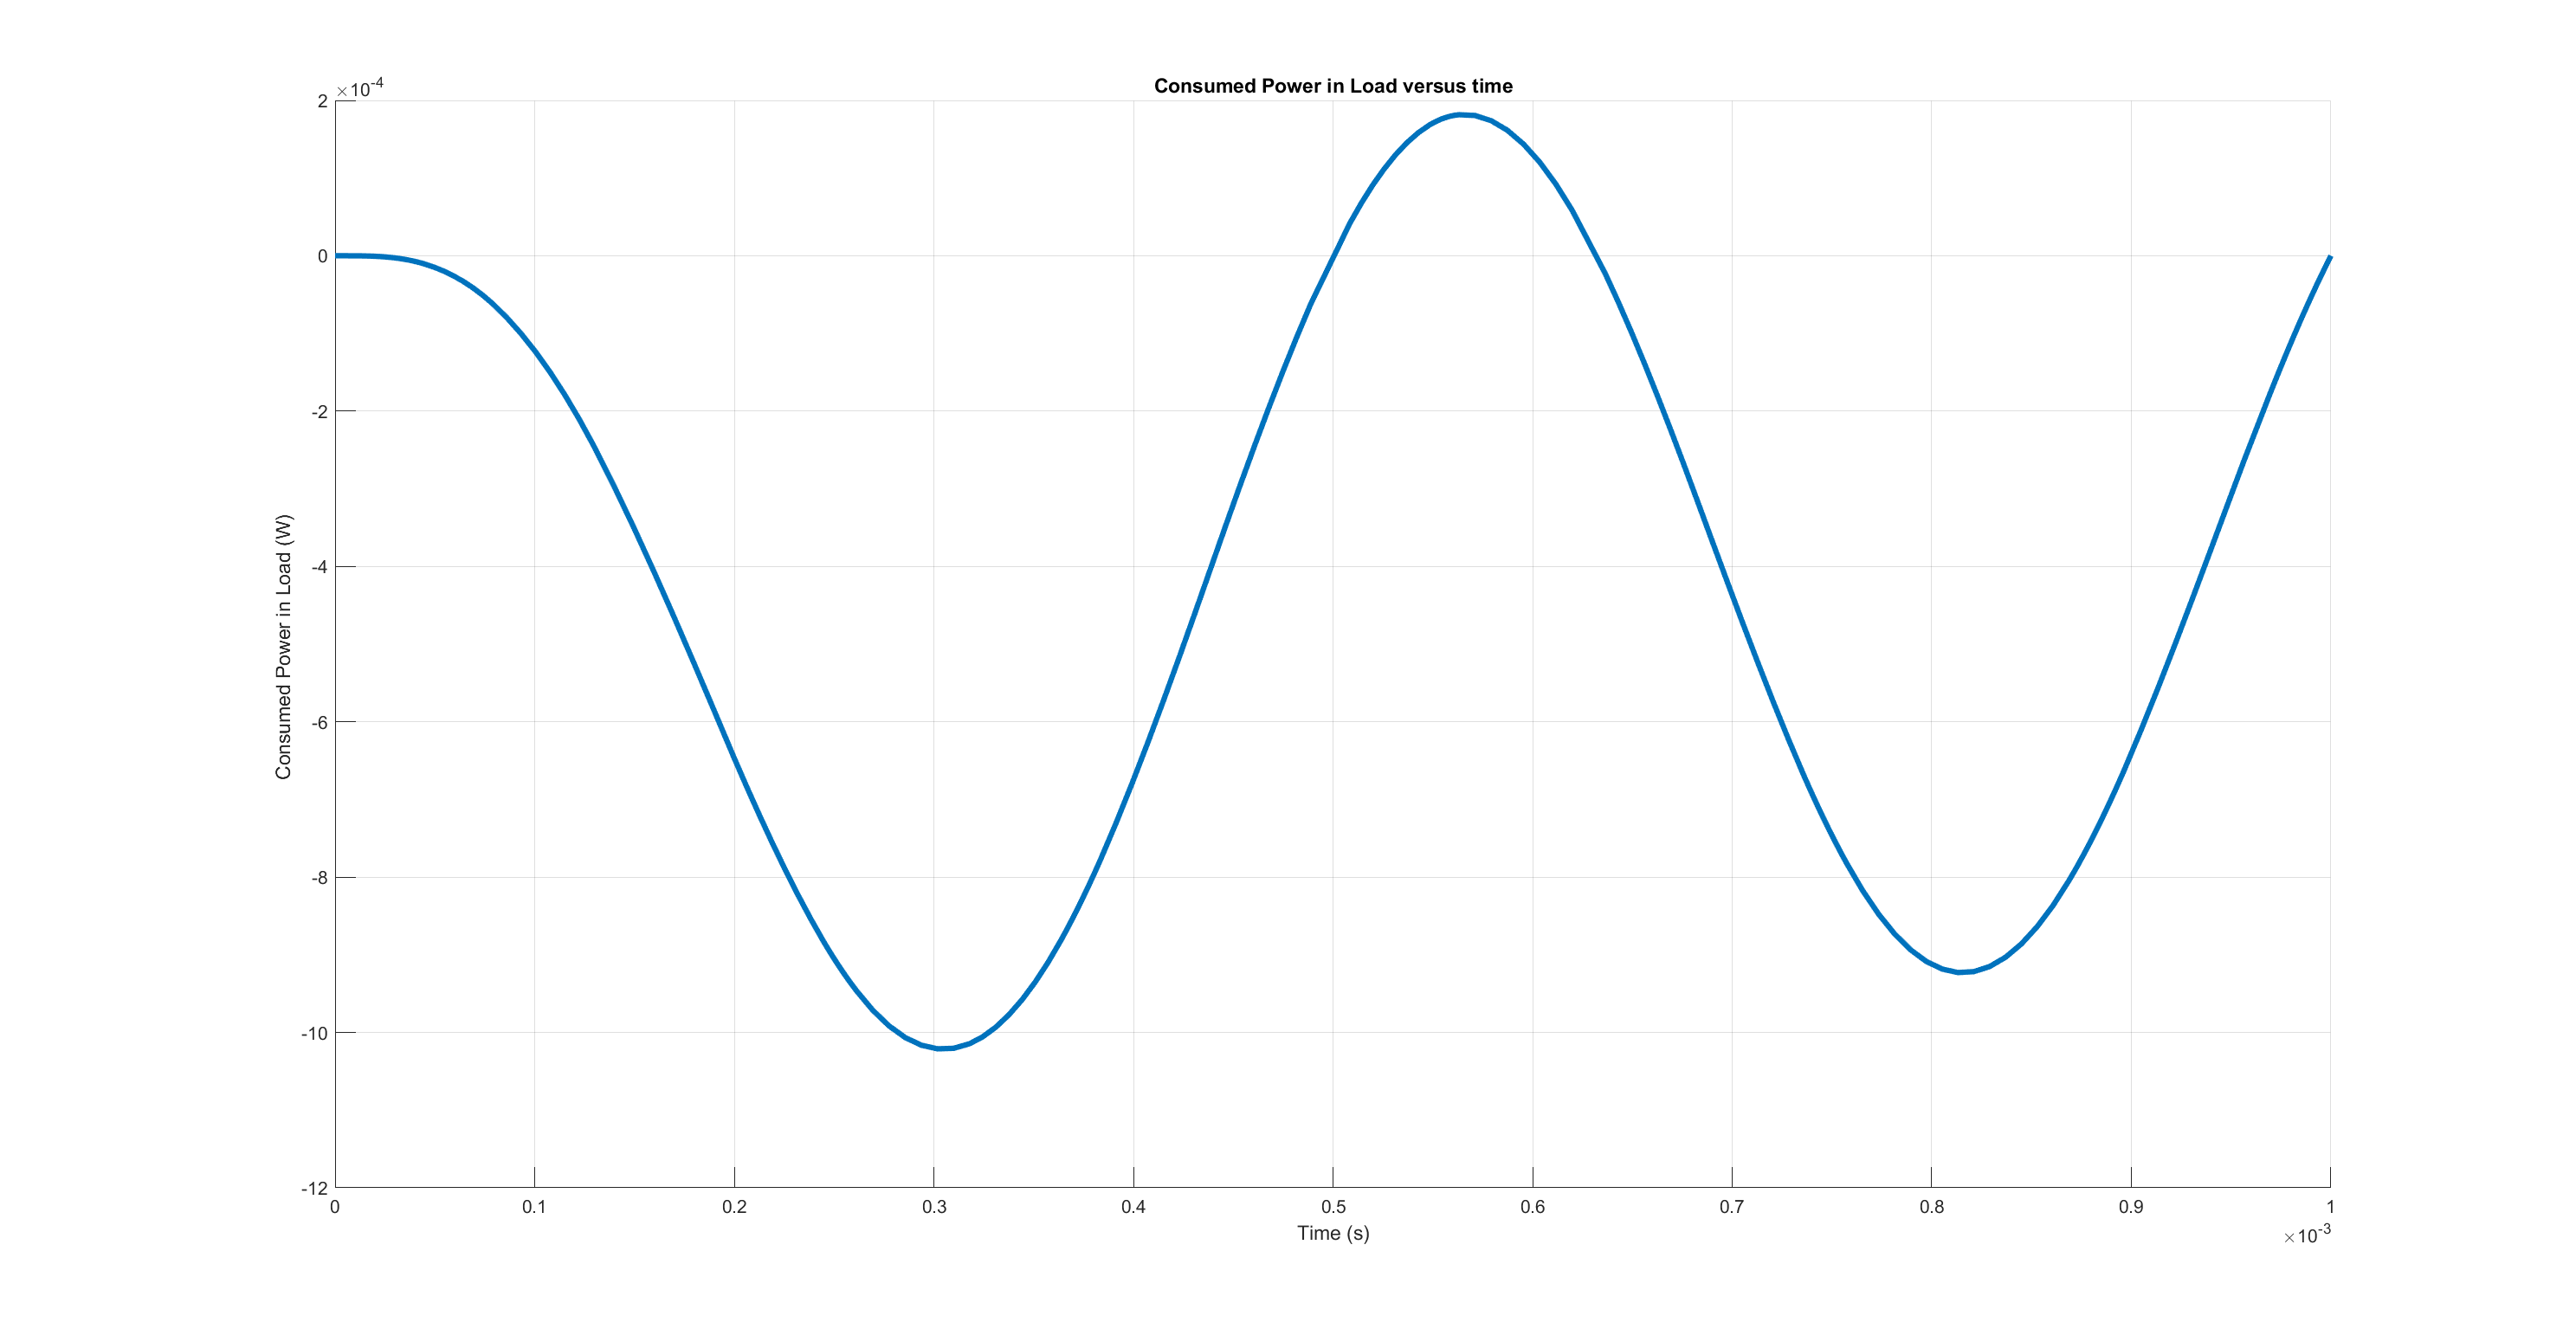
\includegraphics[width=1\textwidth]{2_2.png}
    \caption{Power consumed at load versus Time}
\end{figure} 
The average and the RMS values of the load power are calculated and given in Table 2.
\begin{table}[H]
    \begin{center}
        \caption{Resistance reading by color code convention.}
        \vspace{2mm}
        \begin{tabular}{||c | c ||} 
            \hline
            Average (W) & RMS (W) \\ [0.5ex] 
            \hline\hline
            \(-3.4x10^{-4}\) & \(5.16x10^{-4}\)  \\ 
            \hline
    \end{tabular}
\end{center}
\end{table}

\section{Step 2}
To determine a method to measure the unknown capacitance value C, the circuit given in Figure 8 needed to be constructed.
\begin{figure}[H]
    \centering
    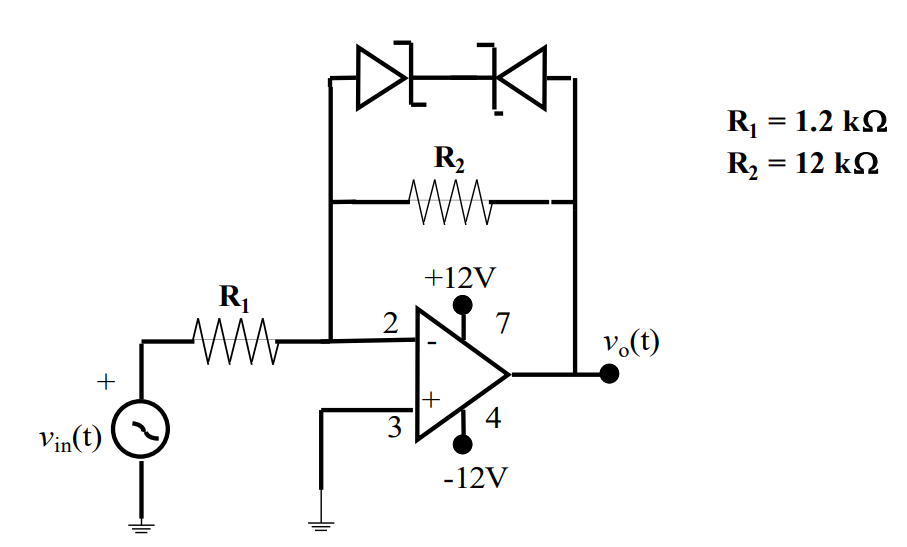
\includegraphics[width=1\textwidth]{2SCH.png}
    \caption{Proposed circuit for Capacitance measurement}
\end{figure} 
Now let us derive the expression for capacitance;


\begin{align*}
    \begin{array}{l}
        V_c(t) = V_m cos(\omega t+ \phi )  \: \Rightarrow  in \: phasors \:  V_m \: \phase {\phi} \\ \\
        i_c(t) = CDV_c(t) = CV_m(-\omega) sin(\omega t + \phi) \\ \\
       = -C\omega V_m cos(\omega t + \phi -90) \\ \\
       =-C\omega V_m \phase {\phi - 90\circ} \\ \\
       V_{in} = V_i  \phase{-90\circ} \\ \\
       Z = \frac{V_c}{I_c} = \frac{V_{in} \phase{\phi}}{ - C \omega V_m \phase{\phi -90 \circ}} = \frac{\phase{90\circ}}{-C\omega} = \frac{J}{-C\omega}  = \frac{1}{j\omega C} \\
       \\
       |Z| = \frac{V}{A} =  \frac{1}{C\omega} \Rightarrow C = \frac{A}{V\omega}
    \end{array}
\end{align*}

\section{Step 3}
To determine a method to measure the unknown inductance value L, the circuit given in Figure 9 needed to be constructed.
\begin{figure}[H]
    \centering
    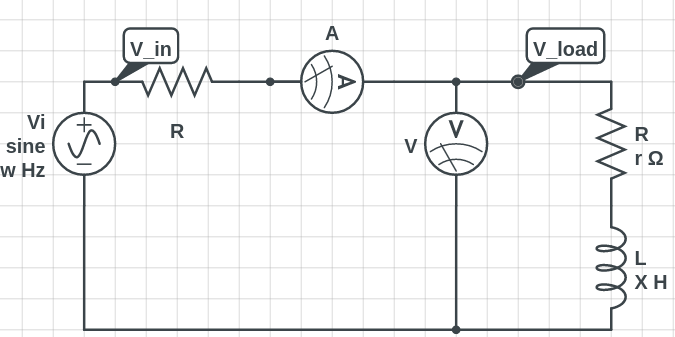
\includegraphics[width=1\textwidth]{3SCH.png}
\caption{Proposed circuit for inductance measurement}
\end{figure} 
Now let us derive the expression for inductance;


\begin{align*}
    \begin{array}{l}
        V_{in}(t) = V_i cos(\omega t+ -90 )  \: \Rightarrow  in \: phasors \:  V_in \: \phase {-90} \\ \\
        Z_L = r + j\omega L \Rightarrow |Z_L| = \sqrt{r^2+\omega^2 L^2} = \frac{V_{rms}}{I_{rms}} \\ \\
        I^2 \omega^2 L^2 = V^2 - I^2 r^2 \\
        So;  \: L = \frac{\sqrt{V_{rms}^2 -  I_{rms}^2 r^2}}{I_{rms} \omega}
    \end{array}
\end{align*}

\section{Step 4}
In this step the circuit schematic given in Figure 10 is the reference.
\begin{figure}[H]
    \centering
    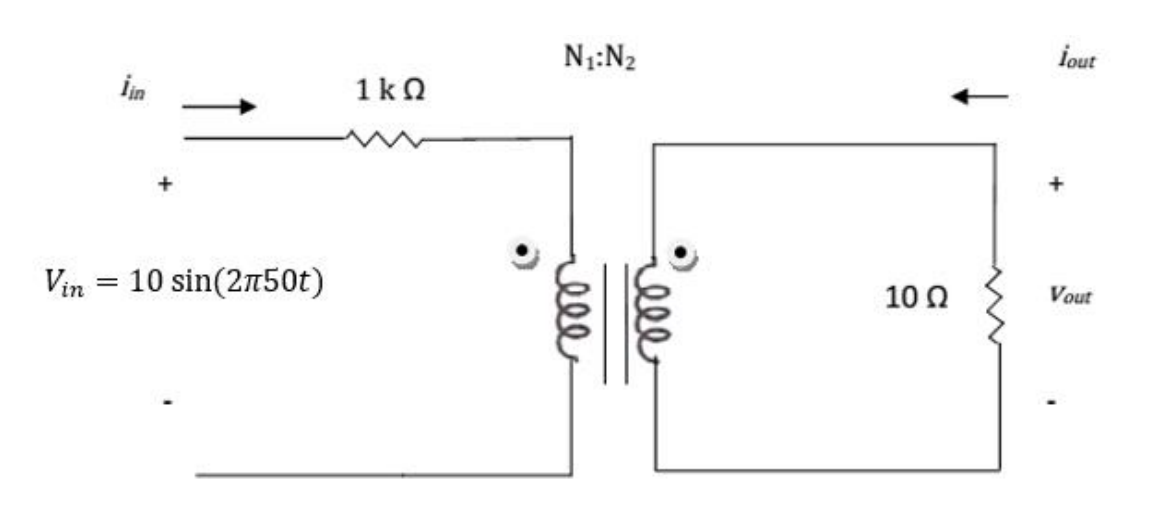
\includegraphics[width=1\textwidth]{4.png}
\caption{Circuit for impedance measurement}
\end{figure} 
\subsection{1st Method}
In first method, the terminal A is denoted as channel 1 and terminal C is denoted as channel 2, terminal B is ground. Here, by inverting the channel 2 in XY mode one can obtain the impedance by dividing the slope by 10. The important thing here is in the signal supply is grounded this method would not work.
\subsection{2nd Method}
In the second method, the terminal A is denoted as channel 1 and terminal B is denoted as channel 2, terminal C is ground. Here one can measure the current by simply dividing the channel 2 by 10 and find the impedance by dividing the channel 1 by the current found. Since it is assumed 10ohm is much smaller than the impedance we could take channel 2 directly. This method can be applied in time mode and phase can be obtained from the measure mode of the DSO directly.

\section{Conclusion}
In this preliminary work document. Neccesssary simuloations concerning complex power are done and plotted. Then some of the measurement techniques for the capacitance , inductance and impedance are examined.

\section*{Appendix A}
The results of the simulations are fetched from LTSpice and plotted in MATLAB in order to make the plots more readable and convenient.


\end{document}

%%%%%%%%%%%%%%%%%%%%%%   EXAMPLE TABLE   %%%%%%%%%%%%%%%%%%%%%%%%%%%%%%%%
\begin{table}[H]
\begin{center}
    \caption{Resistance reading by color code convention.}
    \vspace{2mm}
    \begin{tabular}{||c | c | c||} 
        \hline
        Color Order & Value & Tolerance \\ [0.5ex] 
        \hline\hline
        Brown / Black / Red / Gold & 1k\( \Omega \) & \( \% \) 5  \\ 
        \hline
        Yellow / Violet / Red / Gold & 4.7k\( \Omega \) & \( \% \) 5   \\
        \hline
        Brown / Grey / Orange / Gold & 18k\( \Omega \) & \( \% \) 5  \\ [1ex] 
        \hline
    \end{tabular}
\end{center}
\end{table}


%%%%%%%%%%%%%%%%%%%%%%   EXAMPLE IMAGE   %%%%%%%%%%%%%%%%%%%%%%%%%%%%%%%%
\begin{figure}[H]
\centering
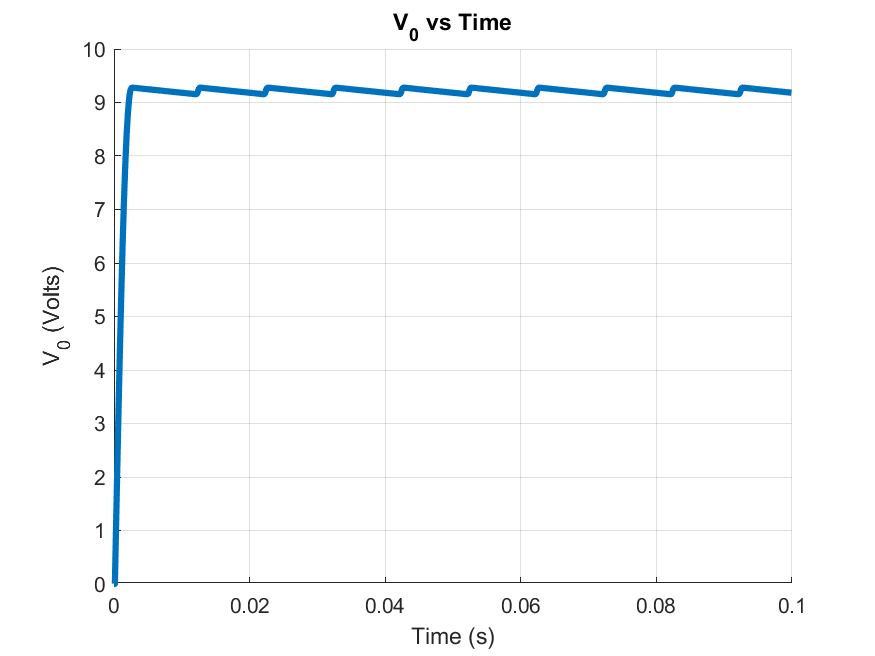
\includegraphics[width=1\textwidth]{5.png}
\caption{Circuit schematic for the step 5}
\end{figure} 

%%%%%%%%%%%%%%%%%%%%%%   EXAMPLE IMAGE FROM PDF   %%%%%%%%%%%%%%%%%%%%%%%%%%%%%%%%
\begin{figure}[H] \centering{
	\includegraphics[scale=0.25]{2a_plot.pdf}}
	\caption{Experiment 2}
\end{figure}
	